\documentclass{article}
\usepackage{amsmath, amssymb, cite, algorithmic, url, braket}
\usepackage{graphicx}
\usepackage{pythonhighlight}
\usepackage[margin=1.5cm]{geometry}
\usepackage[title]{appendix}
\usepackage{listings}
\usepackage{booktabs}
% \usepackage{hyperref}

\graphicspath{{../pic/}}
\lstset{
language=[ANSI]{C},
showtabs=true,
tab=,
tabsize=2,
basicstyle=\ttfamily\footnotesize,%\setstretch{.5},
stringstyle=\color{stringcolour},
showstringspaces=false,
alsoletter={1234567890},
otherkeywords={\%, \}, \{, \&, \|},
keywordstyle=\color{keywordcolour}\bfseries,
upquote=true,
morecomment=[s]{/*}{*/},
commentstyle=\color{commentcolour}\slshape,
literate=*%
{=}{{\literatecolour=}}{1}%
{-}{{\literatecolour-}}{1}%
{+}{{\literatecolour+}}{1}%
{*}{{\literatecolour*}}{1}%
{!}{{\literatecolour!}}{1}%
{[}{{\literatecolour[}}{1}%
{]}{{\literatecolour]}}{1}%
{<}{{\literatecolour<}}{1}%
{>}{{\literatecolour>}}{1}%
% {>>>}{\pythonprompt}{3}%
,%
frame=trbl,
rulecolor=\color{black!40},
backgroundcolor=\color{white},
breakindent=.5\textwidth,frame=single,breaklines=true
}

\begin{document}
\title{DSP Homework 04}
\author{Xu, Minhuan}
\maketitle
\tableofcontents
\begin{abstract}
\subsubsection*{Starlink}
This is a video about how the satellite communicate with the antenna on earth, explaining the 3 questions below.
\begin{enumerate}
    \item How electrical signals become electromagnetic waves
    \item How to realize automatic antenna tracking
    \item How to convert binary data into electrical signal
\end{enumerate}

\subsubsection*{Equation Proof}
We have
$$
s(t) = 
\left\{
    \begin{array}{lr}
        1, & \mathrm{if}\; t = nT,\\
        0, & \mathrm{otherwise.}
    \end{array}
\right.
$$
Prove that
$$
\widetilde{s}(t) = 0
$$

\subsubsection*{Frequency Response of our ears}
This section is mainly about testing our ears with a program written by python.

\subsubsection*{Web Camera}
Monitoring my seat from everywhere on earth.
\end{abstract}

\section{Problem 1}
\subsection{Summary}
\subsubsection{Transmit and Receive}
In order to transmit electrical signals to satellites through wireless channels, we need to convert them into electromagnetic waves. There is a feedline and a metal plate close to each other in the antenna. The electrons will flow quickly (13$~\mathrm{Ghz}$) on the feedline, and the changing electric field will be generated in the process of electron flow. We know that the changing electric field will produce magnetic field, which will finally generate electromagnetic waves. A slice antenna like this will make the electromagnetic wave propagates outwards in a balloon shape.

The single antenna with poor directivity is not what we want, so there are 1280 antennas in the antenna array. Because the phase of electromagnetic wave will change with the position when it is transmitted, there are always constructive interference and destructive interference happening at the same time. This is how the electromagnetic beam is generated.
\subsubsection{Phase Shift}
Due to the unreliability of the motor, it is not unrealistic to use the motor to control the antenna orientation. But, we can change the zone of constructive interference by changing the phase of signal when each antenna emits, so as to change the direction of the beam of electromagnetic wave.
\subsubsection{64QAM}
QAM stands for Quadrature Amplitude Modulation. 64QAM means, on the polar coordinate plane of amplitude-phase, 64 different points are selected to stand for 64 different signals, and each point is encoded with six bit binary. By sending and receiving such high-frequency waves, the antenna can transmit the binary data to the satellites through electromagnetic waves.
\subsection{Further Thoughts}
Starlink is a satellite internet constellation operated by SpaceX, providing satellite Internet access coverage to 40 countries. It also aims for global mobile phone service after 2023.\cite{wiki_starlink}

It looks like a  beautiful vision for the future, everyone on this planet can access the high-speed network. But the price is pretty expensive. The customer's monthly fee is \$99. The cost of dish antennas and routers required to connect satellites is \$549. Whether that vision could achieve success needs to be questioned.

Moreover, this project has brought more problems. Astronomers claim that the number of visible satellites will outnumber visible stars and that their brightness in both optical and radio wavelengths will severely impact scientific observations.\cite{BBC_starlink} With only a speed of 150 and 500Mbit/s, whether this starlink project will change our life, I remain skeptical.

\section{Problem 2}
\subsection{Problem Restatement}
When studying the sampling process, we use the function
\begin{equation}
    s(t) \quad = \quad \left\{ 
        \begin{array}{lr}
            1, & \mathrm{if}\; t = nT,\\
            0, & \mathrm{otherwise.}
        \end{array}
    \right.
    \label{original}
\end{equation}
to express the sampling signal
\begin{align}
    x_s(t) \quad &= \quad x(t)s(t)\\
    &= \quad \left\{
        \begin{array}{lr}
            x(nT), & \mathrm{if}\; t = nT,\\
            0, & \mathrm{otherwise.}
        \end{array}
    \right.
\end{align}
It turns out that such approach is not useful when using the Fourier transform because
\begin{equation}
    \widetilde{s}(f) = \widetilde{x_s}(f) = 0 
    \label{ans}
\end{equation}
Prove (\ref{ans}).
\subsection{Prove}
According to the convolution theorem
\begin{equation*}
    \mathcal{F}\left[ x(t)*y(t) \right] = \widetilde{x}(f) \times \widetilde{y}(f)
\end{equation*}
if 
\begin{equation}
    \widetilde{s}(f) = 0
    \label{sub_ans}
\end{equation}
it's easy to prove Equation \ref{ans}.
I will prove Equation (\ref{sub_ans}) below. Easy to know that
\begin{equation*}
    \widetilde{s}(t) = \int_{-\infty}^{\infty} s(t) e^{-j2\pi ft} \mathrm{d}t
\end{equation*}
Because of Equation (\ref{original})
$$\widetilde{s}(t) = \widetilde{s}(nT) = \sum_{n = -\infty}^{\infty} e^{-j2\pi ft} \mathrm{d}(nT)$$
Because $n \in Z$, threfore
$$
\left\{
    \begin{array}{rl}
    e^{-j2\pi f~nT} = \sin(2\pi f~nT) &- j\cos(2\pi f~nT) < \infty\\
    d(nT) &= 0
    \end{array}
\right.
$$
Therefore
\begin{equation*}
    \widetilde{s}(t) = \sum_{n = -\infty}^{\infty} 0 = 0
\end{equation*}
Therefore
\begin{equation*}
    \widetilde{x}_s(t) = \widetilde{s}(t) = 0
\end{equation*}
Equation (\ref{ans}) proved.

\section{Problem 3}
\subsection{Problem Restatement}
Design and carry out an experiment to find out the highest and lowest audio frequencies that your left and right ears can
hear.
\subsection{Preparation}
I followed the practice of Su Rundong to write a program to generate sound wave (sine wave) of specific frequency, and I think if I can use Qt Designer to generate a program with GUI.

Please look at Fig.\ref{UI}. If I want change the frequency of the sine wave, I can push the buttons or input the frequency I want into the lineEdit box. Push the start button to play the sound.

\begin{figure}[htbp]
    \centering
    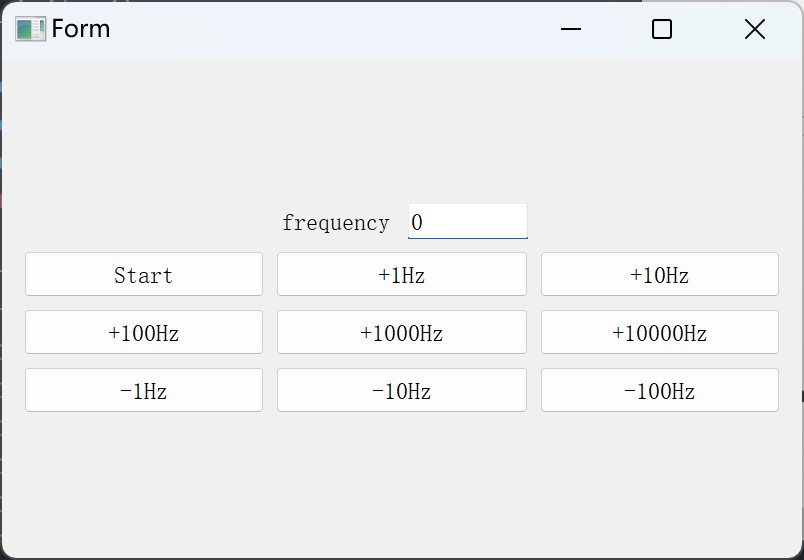
\includegraphics[keepaspectratio,width=250pt]{FreqWindow.jpg}
    \caption{UI of my program}\label{UI}
\end{figure}

\subsection{Interference Factors Elimination}
Earphone makers always tell us that human ears can hear $20-20\mathrm{k}~\mathrm{(Hz)}$. So, I must refer to the instructions of my earphones, and I find that they can only produce sound wave between $20-20\mathrm{k}~\mathrm{(Hz)}$, but actually I can hear some strange sounds if I turn the volumn to maximum. When I am testing my ears with 10$~\mathrm{Hz}$, what I hear cannot be the sound wave of 10$~\mathrm{Hz}$. 

I think it is from the mechanically collision, but I am not sure.To avoid this, I will first make the volumn of my earphones fixed.So I find a website\cite{HearingTest} to test my ears' frequency response, see Fig.\ref{FR}. The position of that black box is higher, I can hear that frequency harder. I don't want to hurt my ears, so I play a sound which is $1\mathrm{~kHz}$, then I will find out the exact range of the frequency my ears can hear in that volumn.

\begin{figure}[htbp]
    \centering
    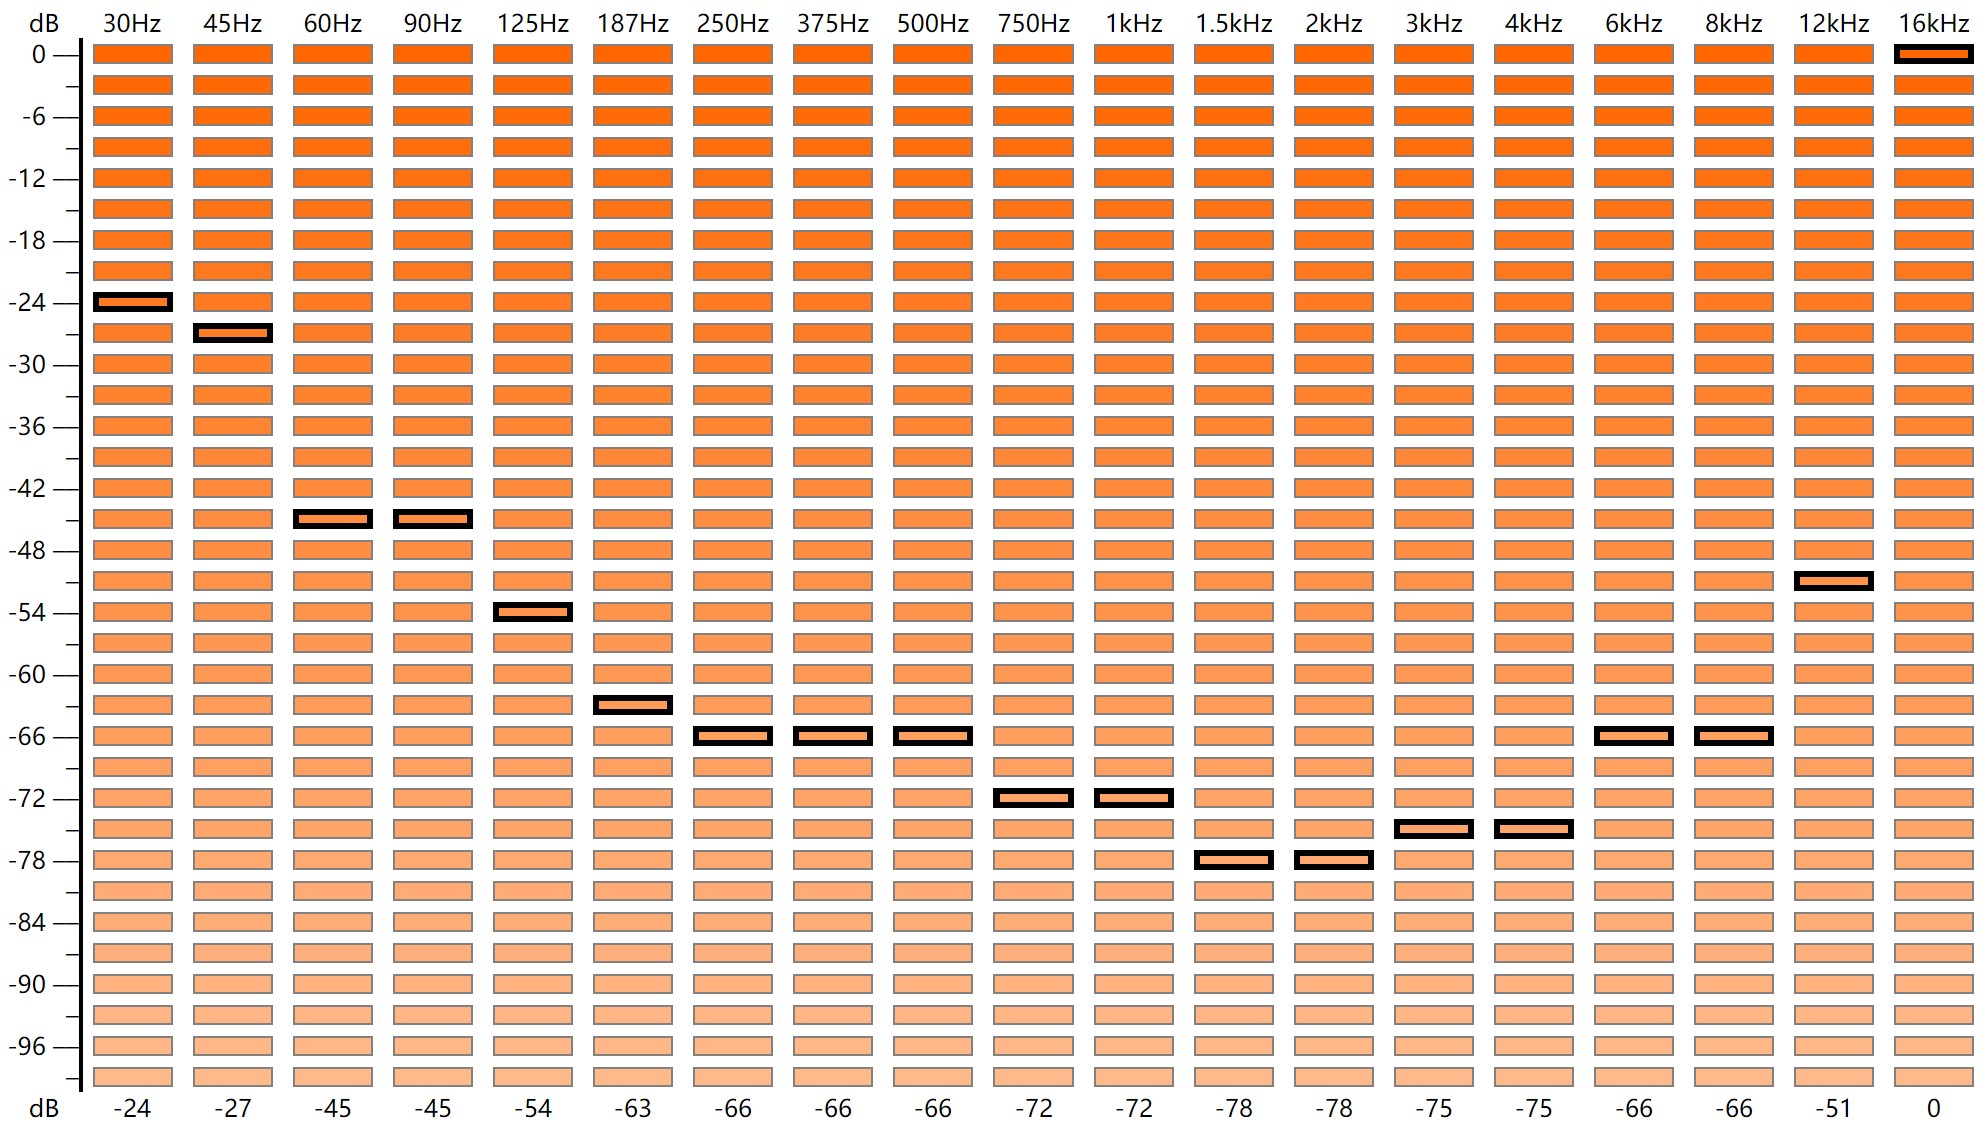
\includegraphics[keepaspectratio,width=400pt]{freqReaction.jpg}
    \caption{Frequency Response}
    \label{FR}
\end{figure}

\subsection{Implement}
From $1~\mathrm{kHz}$, I made the frequency higher and lower until I cannot hear the sound.
At last, in this way, the frequency response range of my ears is $xx \sim xx ~ \mathrm{kHz}$.

\section{Problem 4}
\subsection{Problem Restatement}
Write a (improved) proposal for your first project.
\subsection{Reason}
I bought a Raspberry Pi 4B for fun when I was a freshman, but I don't really have the motivation to use this little thing as something functional. All I did was running a Minecraft server on this thing and broadcast the port where the server ran, in order to play with my friends in other universities.

It costs a lot these days to buy a Raspberry Pi, so I want to make it useful again!
\subsection{Inspiration}
But after I read the proposal of Su Rundong (\emph{He again}), what came into my mind was to let the Raspberry Pi work as the hardware to realize the functions he mentioned in his proposal. Moreover, I want to use this thing as my remote monitor camera so that I can watch my seat and prevent someone from sitting in my chair! (Thankfully, in \emph{LZU}, I have nice roommates who don't mess others' things up)
\subsection{Things I will do}
Raspberry Pi is a rich-functional micro computer, and it can drive camera to record videos or take a photo. What I should do in this project is to 
\begin{enumerate}
    \item Launching a web camera (accessible with Internet) broadcast the live video of my seat in dormitory, like the one in Fig.\ref{webcam}
    \item Using python to control the camera to take a photo
\end{enumerate}
\begin{figure}[htbp]
    \centering
    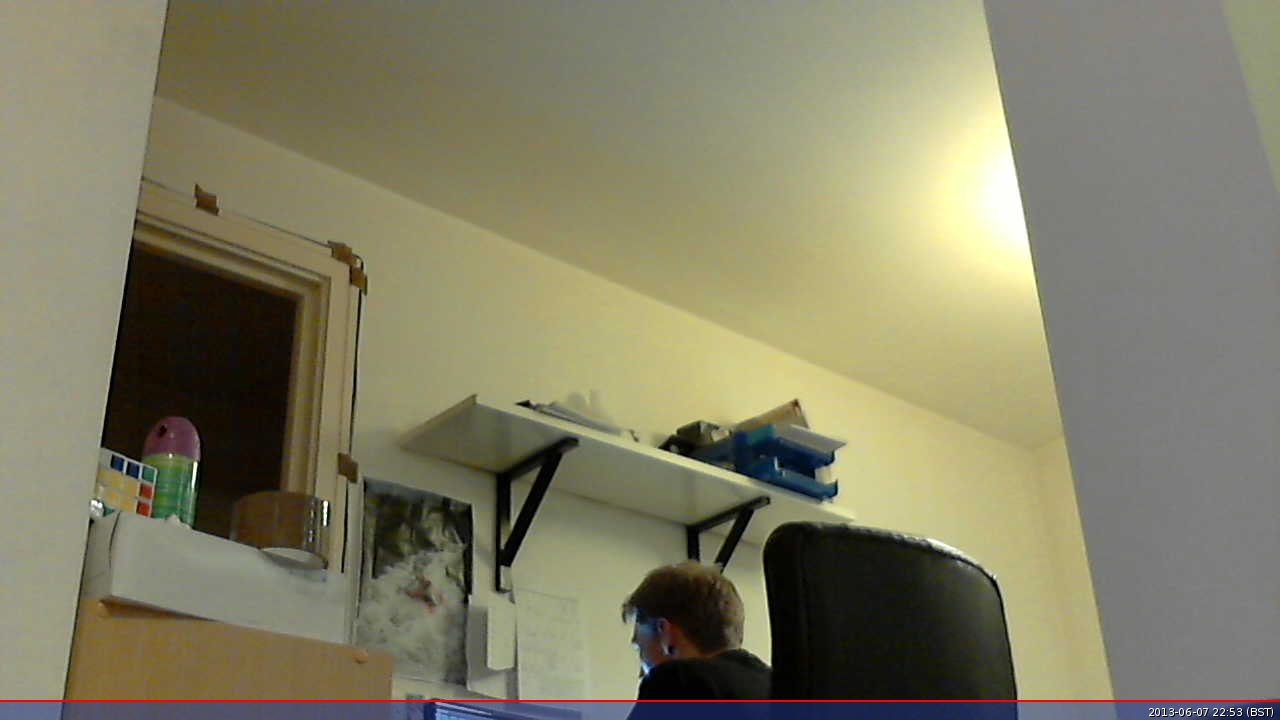
\includegraphics[keepaspectratio,width=250pt]{webcam.jpg}
    \caption{Other people's livestream of the web camera}\label{webcam}
\end{figure}
To achieve the first aim in the last subsection, I will try to use mjpg-streamer\cite{mjpg-streamer} to stream JPEG files over an IP-based network. This is a function already implemented by others, so I will follow the instructions in this repository. The Raspberry Pi will only connect the WiFi in our dormitory, but I will use NAT to broadcast the port so that I can see the video out of dormitory with my smartphone.

Then, the second, it is easy if I use the python package of picamera.
\subsection{Things I will try to do}
A web page that can send http request what tell the camera to take a picture and return with a picture.\cite{web_picam}

\section{Conclusion}
\subsubsection*{Starlink}

Although the starlink project is so amazing, the actual effect of it should be doubted and the problems it brings to us remain to be solved.
\subsubsection*{Equation Proof}

The function 
$$
s(t) = 
\left\{
    \begin{array}{lr}
        1, & \mathrm{if}\; t = nT,\\
        0, & \mathrm{otherwise.}
    \end{array}
\right.
$$
is not suitable for sampling.
\subsubsection*{Frequency Response of our ears}

My left ears can hear $xx \sim xx ~ \mathrm{kHz}$ sound waves and my right ears can hear $xx \sim xx ~ \mathrm{kHz}$ sound waves.
\subsubsection*{Web Camera}

I'll try to launch a web camera with Raspberry Pi which is connected to the Internet.
\bibliographystyle{ieeetr}
\bibliography{../bib/database}

\begin{appendices}
    \section{Code Listing}
    \begin{python}
    # main.py
    from PyQt5.QtWidgets import QApplication, QWidget
    import sys
    import sounddevice as sd
    import numpy as np
    from form import Ui_Form #a form auto-generated from a ui file which was made in help of Qt Creator

    class FormWidget(QWidget):
        def __init__(self):
            super().__init__()
            self.ui = Ui_Form()
            self.ui.setupUi(self)
            self.ui.retranslateUi(self) #initialize the ui
            self.Ui_connect() #connect buttons with functions
            self.ui.freq_le.setText('0') #initial value of frequency
        
        def Ui_connect(self):
            self.ui.start.pressed.connect(self.toPlay)
            self.ui.m1.pressed.connect(self.addFreq)
            self.ui.m10.pressed.connect(self.addFreq)
            self.ui.m100.pressed.connect(self.addFreq)
            self.ui.p1.pressed.connect(self.addFreq)
            self.ui.p10.pressed.connect(self.addFreq)
            self.ui.p100.pressed.connect(self.addFreq)
            self.ui.p1000.pressed.connect(self.addFreq)
            self.ui.p10000.pressed.connect(self.addFreq)

        def toPlay(self):
            '''
            Generate and play the sound wave according to the text of lineEdit.
            '''
            f = int(self.ui.freq_le.text()) # frequency of the sine wave
            fs = 96000 # sampling 
            length = 10 # seconds it lasts
            x = np.arange(fs*length)
            y = np.sin(2 * np.pi * f / fs * x) # generate a sine wave
            sd.play(y,fs,blocking=False) # play the sine wave as a sound wave
            
        def addFreq(self):
            '''
            Increase or decrease the value in LineEdit which stands for the frequency of sound wave
            '''
            sender = self.sender()
            sender_name = sender.objectName()
            try:
                f = int(self.ui.freq_le.text()) # get the value of LineEdit
            except:
                self.ui.freq_le.setText('0') # default frequency (be 0 for protecting ears)
                f = 1
            if sender_name == 'm1':
                f = f - 1
            elif sender_name == 'm10':
                f = f - 10
            elif sender_name == 'm100':
                f = f - 100
            elif sender_name == 'p1':
                f = f + 1
            elif sender_name == 'p10':
                f = f + 10
            elif sender_name == 'p100':
                f = f + 100
            elif sender_name == 'p1000':
                f = f + 1000
            else:
                f = f + 10000
            self.ui.freq_le.setText(str(f)) # show the changed frequency
            

    if __name__ == '__main__':
        app = QApplication(sys.argv)
        main = FormWidget()
        main.show() #initialize and show the window
        sys.exit(app.exec_())
    \end{python}
    \begin{python}
    #form.py

    
    # -*- coding: utf-8 -*-

    # Form implementation generated from reading ui file 'form.ui'
    #
    # Created by: PyQt5 UI code generator 5.15.7
    #
    # WARNING: Any manual changes made to this file will be lost when pyuic5 is
    # run again.  Do not edit this file unless you know what you are doing.


    from PyQt5 import QtCore, QtGui, QtWidgets


    class Ui_Form(object):
        def setupUi(self, Form):
            Form.setObjectName("Form")
            Form.resize(800, 500)
            self.verticalLayout = QtWidgets.QVBoxLayout(Form)
            self.verticalLayout.setObjectName("verticalLayout")
            self.gridLayout = QtWidgets.QGridLayout()
            self.gridLayout.setObjectName("gridLayout")
            self.freq_lb = QtWidgets.QLabel(Form)
            self.freq_lb.setAlignment(QtCore.Qt.AlignCenter)
            self.freq_lb.setObjectName("freq_lb")
            self.gridLayout.addWidget(self.freq_lb, 0, 1, 1, 1)
            self.freq_le = QtWidgets.QLineEdit(Form)
            self.freq_le.setObjectName("freq_le")
            self.gridLayout.addWidget(self.freq_le, 0, 2, 1, 1)
            self.start = QtWidgets.QPushButton(Form)
            self.start.setObjectName("start")
            self.gridLayout.addWidget(self.start, 1, 0, 1, 1)
            self.p1 = QtWidgets.QPushButton(Form)
            self.p1.setObjectName("p1")
            self.gridLayout.addWidget(self.p1, 1, 1, 1, 2)
            self.p10 = QtWidgets.QPushButton(Form)
            self.p10.setObjectName("p10")
            self.gridLayout.addWidget(self.p10, 1, 3, 1, 1)
            self.m1 = QtWidgets.QPushButton(Form)
            self.m1.setObjectName("m1")
            self.gridLayout.addWidget(self.m1, 3, 0, 1, 1)
            self.p100 = QtWidgets.QPushButton(Form)
            self.p100.setObjectName("p100")
            self.gridLayout.addWidget(self.p100, 2, 0, 1, 1)
            self.p1000 = QtWidgets.QPushButton(Form)
            self.p1000.setObjectName("p1000")
            self.gridLayout.addWidget(self.p1000, 2, 1, 1, 2)
            self.p10000 = QtWidgets.QPushButton(Form)
            self.p10000.setObjectName("p10000")
            self.gridLayout.addWidget(self.p10000, 2, 3, 1, 1)
            self.m10 = QtWidgets.QPushButton(Form)
            self.m10.setObjectName("m10")
            self.gridLayout.addWidget(self.m10, 3, 1, 1, 2)
            self.m100 = QtWidgets.QPushButton(Form)
            self.m100.setObjectName("m100")
            self.gridLayout.addWidget(self.m100, 3, 3, 1, 1)
            self.gridLayout.setColumnStretch(0, 2)
            self.gridLayout.setColumnStretch(1, 1)
            self.gridLayout.setColumnStretch(2, 1)
            self.gridLayout.setColumnStretch(3, 2)
            self.verticalLayout.addLayout(self.gridLayout)

            self.retranslateUi(Form)
            QtCore.QMetaObject.connectSlotsByName(Form)

        def retranslateUi(self, Form):
            _translate = QtCore.QCoreApplication.translate
            Form.setWindowTitle(_translate("Form", "Form"))
            self.freq_lb.setText(_translate("Form", "frequency"))
            self.start.setText(_translate("Form", "Start"))
            self.p1.setText(_translate("Form", "+1Hz"))
            self.p10.setText(_translate("Form", "+10Hz"))
            self.m1.setText(_translate("Form", "-1Hz"))
            self.p100.setText(_translate("Form", "+100Hz"))
            self.p1000.setText(_translate("Form", "+1000Hz"))
            self.p10000.setText(_translate("Form", "+10000Hz"))
            self.m10.setText(_translate("Form", "-10Hz"))
            self.m100.setText(_translate("Form", "-100Hz"))
    \end{python}
\end{appendices}

\end{document}

